\documentclass[../main.tex]{subfiles}
\graphicspath{{\subfix{../images/}}}
\begin{document}

\subsubsection{Posterising}

\begin{figure}[h!]
  \centering
  \begin{subfigure}[b]{0.5\linewidth}
    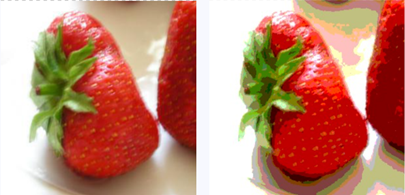
\includegraphics[width=\linewidth]{strawberry.png}
  \end{subfigure}
  \caption{Strawberry Images with Posterising}
  \label{fig:strawberry-postering-edit}
\end{figure}

\begin{figure}[h!]
  \centering
  \begin{subfigure}[b]{0.5\linewidth}
    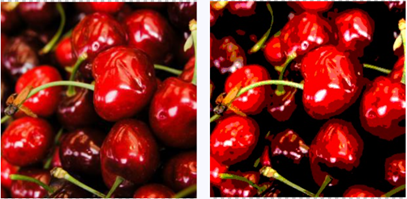
\includegraphics[width=\linewidth]{cherry.png}
  \end{subfigure}
  \caption{Cherry Images with Posterising}
  \label{fig:cherry-postering-edit}
\end{figure}

Posterise our images means to group pixels together to have a single color. This helps to separate individual colours that are in the image. Posterising can also help the model notice how the skin reacts to light. 
Strawberries have a bumpy surface due to its seeds on its skin which causes the surface to be less reflective. Posterising the image will show fewer color groups and will be more matte. 
Cherries have a reflective skin so light bounces off it to show highlights and areas of brighter colouring. 

\end{document}